\Chapter{Tesztelés}

\section{Az alkalmazás elindítása}

Az alkalmazás elindításakor megjelenik a \textit{Main Menu} kiírás, ezen az oldalon, közép lent lévő ként opció közül választhatunk,
a fel és lefele nyilak segítségével, a kiválasztott menü pont alatt egy aláhúzás fog megjelenni,
amely a felhasználó számára jelzi, hogy melyik menü pont a jelenleg kiválasztott.

A számunkra megfelelő menüpont kiválasztása utána az \texttt{Enter} lenyomásával véglegesíthetjük döntésünket.
Ekkor a menüpontnak megfelelő utasítás fog végrehajtódni.

Ha a \textit{Start} menüpontot választottuk, akkor elhagyjuk a főmenüt és elkezdődik a szimuláció.
Ha a \textit{Quit} menüpontot választottuk, akkor az alkalmazás bezáródik.

\Section{Szimuláció közben használható funkciók}

\subsection{Pause}
A szimuláció közben a felhasználónak lehetősége van megállítani a szimulációt, hogyha megszeretne valami vizsgálni vagy csak
megszeretné állítani ideiglenesen a szimulációt. Ezt a \texttt{P} gomb megnyomásával teheti meg.

Az alkalmazás a szimuláció megállását, a bal felső sarokban kiírt fehér \textit{Paused} felirattal jelzi a felhasználó számára.
Ha a szimuláció jelenleg meg van állítva, akkor a \texttt{P} gomb még egyszer megnyomásával újra elindíthatjuk azt.

\subsection{Statistics ablak}
A szimuláció szüneteltetésétől függetlenül bármikor megnyithatjuk egy ágens \textit{Statistics} oldalát, ahol mindig az első ágens adait fogjuk látni először.
Megnyitása és bezárása a \texttt{C} gomb lenyomásával lehetséges.
Ez az ablak 6 darab sort tartalmaz, mindegyik az ágens egy adatát írja ki a felhasználó számára.
Az ágensek között a \texttt{Q} és \texttt{E} gombok megnyomásával haladhatunk hátra és előre. Az alkalmazás ezek használatára az ágens ablak bal alsó és jobb alsó
sarkában lévő \textit{PRESS Q} és \textit{PRESS E} kiírásokkal vonja fel a felhasználó figyelmét.

\subsection{Inventory ablak}
A \textit{Statistics} ablakban megjelenített ágensnek sorszámától és a szimuláció szüneteltetésétől függetlenül bármikor megnyithatjuk a hozzá tartozó \textit{Inventory} ablakot.
Ezt az ablakot az ágens ablakkal ellentétben nem lehet léptetni, mindig a \textit{Statistics} ablakban vizsgált ágens \textit{Inventory} adatait fogja kiírni.
Ezt az ablakot önmagában nem lehet megnyitni, csak akkor ha már a \textit{Statistics} ablak meg van nyitva.
Megnyitása és bezárása az \texttt{I} gomb lenyomásával lehetséges.
Ez az ablak tartalmaz 8 négyzetet és egy rövid tárgy leírást, amely lehet 1 vagy 6 sorú, a tárgy típusától függően. Ha a tárgy hordható típusú, akkor első sorában a nevét, 
a további 4 sorában a statisztikáit láthatjuk, majd végül az utolsó sorában azt hogy fel van-e szerelve az ágens által. Ha a tárgy nem hordható (kulcs), 
akkor a tárgy leírásában csak az első sorát, a nevét fogjuk látni.
Az ablak megnyitásakor mindig a bal felső négyzet van kijelölve, amelyet az alkalmazás úgy jelöl a felhasználó számára, hogy egy fehér négyzetet helyez rá.
A négyzetekben tárgyak képeit láthatjuk, hogy ha a vizsgált ágens \textit{Inventory} listája tartalmaz valamilyen tárgyat.

\Section{Szimuláció vége}

A szimuláció befejeződésekor a képernyő közepén láthatunk egy kiírást, amelyben a szín attól függ, hogy mely csapat nyerte a szimulációt.

\Section{Eredmények}

Ez a szakasz arról fog beszámolni, hogy milyen utat jártak be az ágensek két különböző szimulációban. Az általuk bejárható területeket a \aref{fig:map}. ábrán mutatom be. Minden fehér négyzet azt a területet ábrázolja, amelyet az ágens képes bejárni, amíg a narancssárga minden olyan területet mutat, amit semmilyen esetben nem tud bejárni. 

\begin{figure}[!ht]
    \centering
    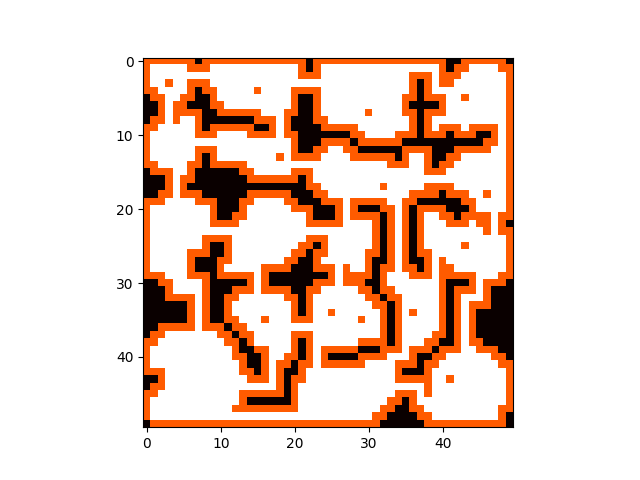
\includegraphics[scale=0.7]{images/map.png}
    \caption{Map}
    \label{fig:map}
\end{figure}

\begin{figure}[h!]
    \begin{center}
        \begin{tabular}{cc}
            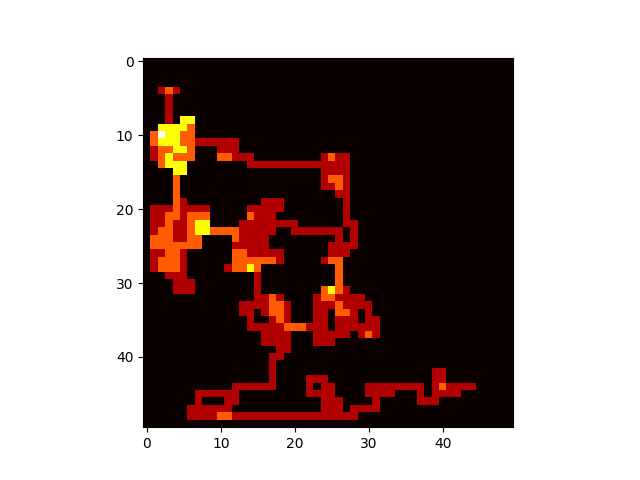
\includegraphics[width=0.45\textwidth, height=60mm]{images/test1_agent1.png}
            & 
            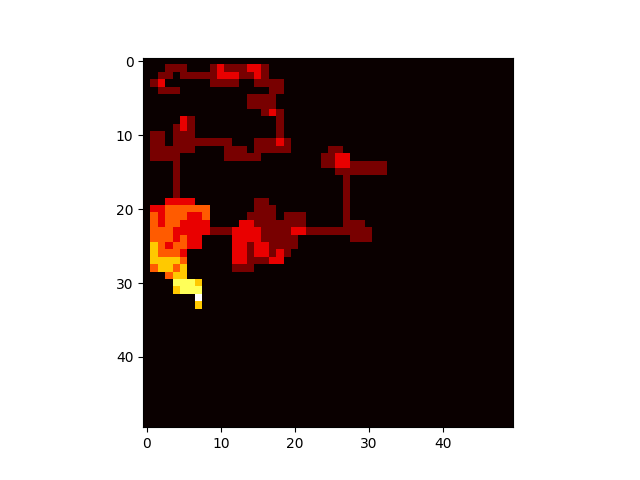
\includegraphics[width=0.45\textwidth, height=60mm]{images/test2_agent1.png}    
            \\
            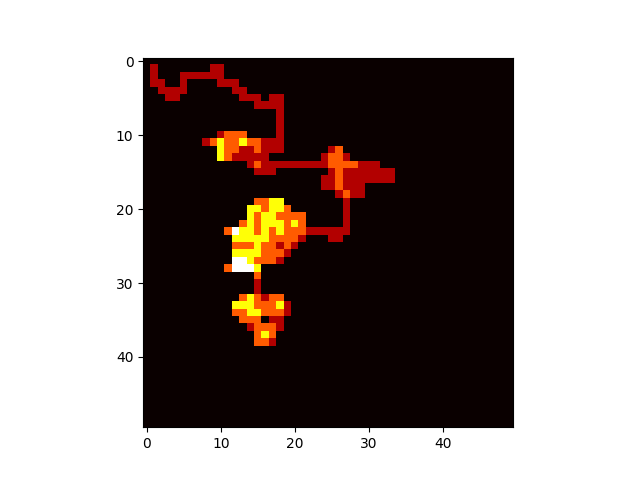
\includegraphics[width=0.45\textwidth, height=60mm]{images/test1_agent2.png}
            &
            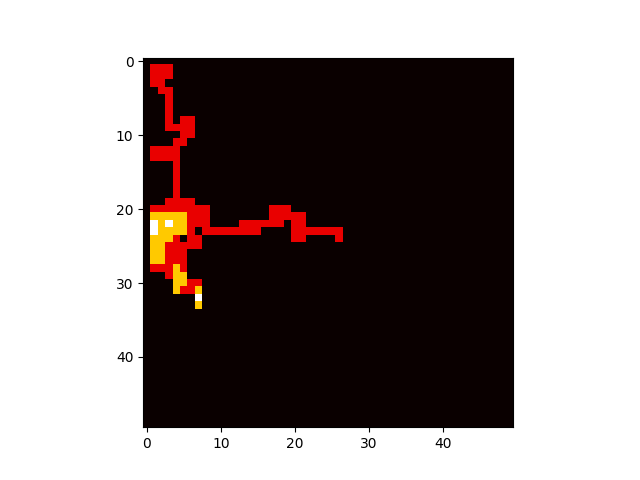
\includegraphics[width=0.45\textwidth, height=60mm]{images/test2_agent2.png}
            \\
            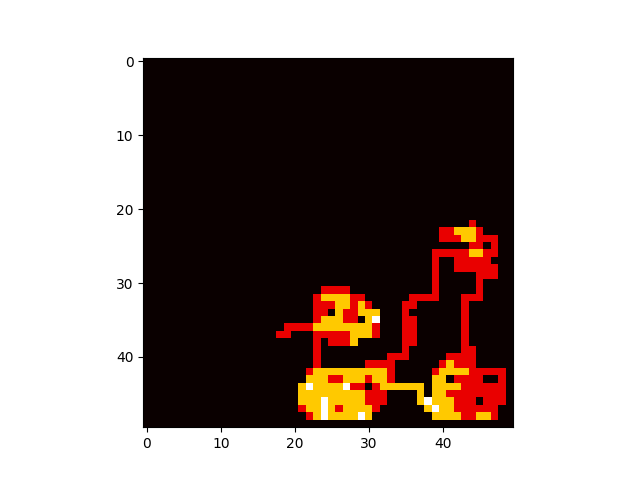
\includegraphics[width=0.45\textwidth, height=60mm]{images/test1_agent3.png}    
            & 
            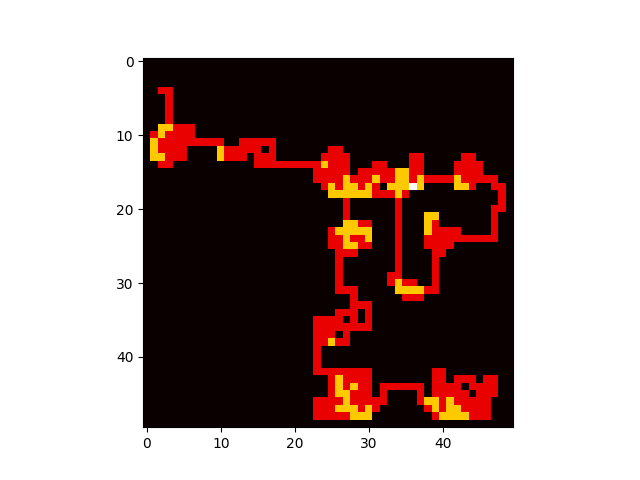
\includegraphics[width=0.45\textwidth, height=60mm]{images/test2_agent3.png}
            \\
            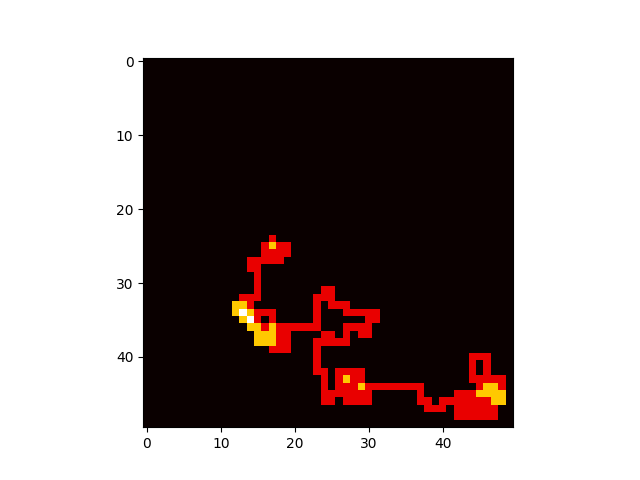
\includegraphics[width=0.45\textwidth, height=60mm]{images/test1_agent4.png}    
            & 
            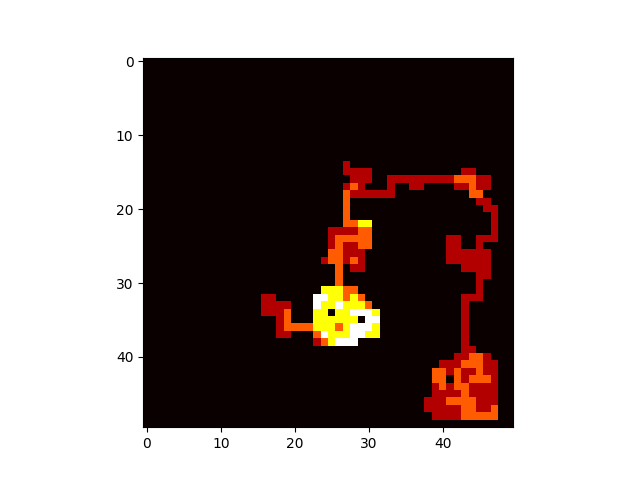
\includegraphics[width=0.45\textwidth, height=60mm]{images/test2_agent4.png}
            \\
        \end{tabular}
        \caption{Teszt eredmények}
        \label{tbl:tests}
    \end{center}
\end{figure}

Két szimulációban kapott eredményeket mutatom be a következő \ref{tbl:tests}. ábrán. Minden oszlop egy különálló szimuláció eredményeit ábrázolja. 
Itt látható, hogy mely ágens mely szimulációban milyen utat járt be a mapon. Mivel az eredményeket bemutató ábrákat \textit{heapmap}-eknek nevezzük, ezért egy adott blokk minél többször bejárt annál jobban fog kifehéredni.

Az ágensek mozgását befolyásolták általuk megtalált tárgyak, ellenséges ágensek és bezárt ajtók.

A képeken látszódnak szobák belsejében néhol egy vagy két fekete négyzet, ezek a szobákban lévő mozgást korlátozó oszlopok miatt vannak, amely megakadályozzák az ágenseket, hogy az adott négyzetekre lépjenek.

Mozgást korlátozó objektumok lehelyezése azért volt célszerű, hogy megakadályozzam néhány esetben azt, hogy az ágens néhány tárgyat könnyen észrevegyen.
